\chapter{ Foundations} \label{foundations}
This project uses the Genode operating system framework with the L4/Fiasco kernel. Since the kernel itself acts a type-I Hypervisor, which allows for partitioning of different software components via separated container, making them work on user mode level \cite{kia4sm}.

To understand the design and implementation of this project, the reader has to be aware of few important concepts related to both Genode operating system and L4 Fiasco.OC kernel. Many concepts explained here are based on ideas from the Genode book \cite{genodebook}, so they are not explained in detail.

\section{Genode Operating System Framework} \label{foundations_genode}
The Genode operating system framework is a tool kit for building secure and special purpose operating systems. Genode is maintained by the German company, Genode Labs GmbH, which  offers both commercial licenses  and open-source license under GPLv2. The operating system can be used as an embedded operating system or a fully sophisticated general purpose operating system. 

The Genode operating system uses a recursive tree structure, where each node in the tree represents a component. Each node is owned by its parent, which controls every aspect of its child like resource control and execution environment. The root of the tree is a minimalistic microkernel, which is responsible for providing protection domain, threads of execution and communication mechanism between the protection domains. The rest of the operating system's features, such as the device drivers, network stacks, file systems, virtual machines are the nodes of the operating system. Each component gets a share of the physical resources available. The components can grant the resources to their children. If a components wants additional resources, it can request its parent, and the parent can grant or deny it.

The above features make Genode operating system have a smaller trusted computing base(TCB) and give better security features. If a parent component thinks that a child is compromised, it can destroy the child while keeping the rest of the system safe. Genode operating system has been developed to strike a balance between various aspects of different operating systems. For example, the OS has to provide an assurance that threads get fair share of execution time while accommodating rich and dynamic workloads. A similar mechanism is employed for providing security features and user friendliness.

Genode supports both x86 and ARM CPU architectures, and can be used with most members of the L4 family(NOVA, Fiasco.OC, OKL4 v2.1, L4ka::Pistachio, Codezero and L4/Fiasco) of micro kernels. On the Fiasco.OC, Genode supports paravirtualization, which is a virtualization technique that provides an interface to virtual machines that are similar to their underlying hardware. This method can be effectively used to solve safety related issues of mixed-criticality systems such as the one presented in the KIA4SM project. Hence, it makes a very good choice of operating system to use for the KIA4SM project.

\subsection{Source Tree Structure}
At the root of the directory, there are 3 folders- \texttt{doc/}, which contains the documentation of and the release notes of all versions, \texttt{tool/} folder for build systems and tools used in the system, and \texttt{repos/}, which contains the source-code repositories. 

Inside the \texttt{repos/} folder, \texttt{base/} repository contains the basic framework related code. The \texttt{base-<platform>/} folders contain the platform specific code, where <platform> refers to the microkernel name. For example, \textit{foc} contains the code for the Fiasco.OC.

\subsection{Capabilities, RPC Objects, Protection Domain}\label{Foundations:cap}
Genode consists of many components, and each component lives in a \texttt{protection domain}, which provides an isolated execution environment. The resource is abstracted to an \texttt{RPC object} and a token that gives access to this RPC object is called \texttt{Capability}.

When an RPC object is created, Genode creates a so-called \texttt{object-identity}, which represents the RPC object in the kernel space. The kernel maintains a capability space, which holds reference for the object identities. This capability space is explained in detail in \ref{founcations:overfiasco}. The capabilities can be passed to different components, and this operation of transferring capability from one protection domain to another is called  \texttt{delegation}.

\subsection{Client-Server Relationship}
Capabilities are used to call methods of RPC objects that are from different protection domains. The component that uses the RPC object is called client and the owner of the RPC object plays the role of the server. The server should at-least have one thread called \texttt{entrypoint}, which gets activated when the client calls the method.

Clients generally have to trust the server since they are granted from the parent through session invocation. Servers that do not trust their clients can cancel the service anytime if they detect a security threat.

 
\subsection{Component Creation}
Genode component is made up of five basic parts, 

\begin{labeling}{component}
\item[RAM session] Allocates memory for a program's BSS and heap
\item[ROM session] Contains an executable binary
\item[CPU session] Creates an initial thread of the component
\item[RM session] Manages the component's address space 
\item[PD session] Represents the protection domain
\end{labeling}

As mentioned earlier each Genode component is created out of a parent, which is responsible for granting these sessions to child. 

\subsection{Inter-component Communication}\label{Foundations:icc}
Genode provides three principle mechanisms for inter-component communication namely, synchronous remote procedure calls (RPC), asynchronous notifications and shared memory. Synchronous RPC is the prominently used communication mechanism in the Genode world, since this not only able to transfer the information, but also has the ability to delegate the capabilities and has the system-wide authority. 
RPC mechanism is similar to a way a function calls work, where control transfer between caller and callee happens. Synchronous RPC mechanism uses kernel's IPC to transfer messages between a client and the server. The asynchronous notification is helpful when the caller doesn't want to wait for the control to come back. The Synchronous RPC mechanism was considered for use in this work, but this is not useful in cases of bulk transfer of data between Controller and Synchronization component. So, the idea of Shared memory concept came as a replacement.

The steps taken in allocating and using shared dataspace are,
\begin{enumerate}
\item The first step is to allocate the memory. The server does this by interacting with the core's RAM service to allocate a new RAM dataspace. This space is owned by the server.

\item The server attaches the dataspace to its own RM session. This makes the dataspace contents available in its virtual address space.

\item Server delegates the authority to a client whenever a request for the dataspace is made.

\item The client can attach the obtained dataspace from the server to its own RM session to access the contents.
\end{enumerate}

All of these methods are rarely used in isolation and most of the communication methods are used in combination of these methods. In this particular work, RPC and shared memory were used in combination.

\subsection{Interaction with the Kernel}
The interaction of user-level threads with the kernel can be seen as a state machine with state transitions. The user-level threads in Genode enter the kernel via a system call, either by device interrupts or by a CPU exception. Once entered, the kernel takes the corresponding action for the event that caused the kernel entry, and the thread leaves the kernel to the user-space.

One such kernel interaction is scheduling a thread. Scheduler maintains a list of so-called scheduling contexts and each of these refers to a thread. Each time the kernel is entered, the scheduler is updated with the passed duration. When updated, it takes a scheduling decision by making the next to-be-executed thread the head of the list. At kernel exit, the control is passed to the user-level thread that corresponds to the head of the scheduler list.

\subsection{Trace Service}
Genode has a Trace service, which can be used by the user-level components for light weight event-tracing. This can be used for obtaining the thread related information for all the threads available in the system. This service is used in the testing of the thread update mechanism which will be explained later in chapter \ref{chap:testing}.

\section{Overview of L4/Fiacso.OC} \label{founcations:overfiasco}
Fiasco.OC is a 3rd generation capability-based microkernel, which belongs to the L4 family of microkernels. Fiasco provides multi-processor support, hardware assisted virtualization and paravirtualization. It is capable of real-time scheduling and is scalable from embedded to HPC systems \cite{foc_feat}. These features made Fiasco.OC the ideal choice for using in this project. Fiasco.OC can used with the L4 Runtime Environment (L4Re), which provides the necessary support to develop applications, or with an operating system such as Genode.

The OC in Fiasco.OC stands for Object-Capability system. In this kernel, everything is represented as an object and the objects interact with each other with a kernel provided IPC mechanism. Each object provides services that other objects can use. The capabilities in the Fiasco.OC represents references to the kernel objects and are stored in a per task capability mapping tables, which increases the security of the kernel. The figure \ref{fig:foc_cap} \cite{foc_pdf}, shows the per-task capability table. The kernel also provides a factory for object management.

\begin{figure}[h]
\centering
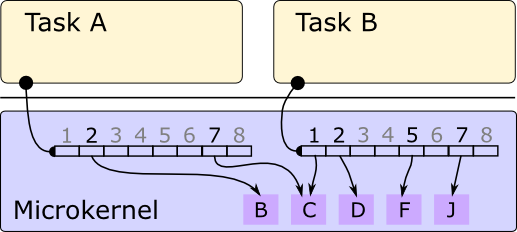
\includegraphics[width=0.7\linewidth]{figures/foc_cap.png}
\caption {Per process capability table in Fiasco.OC \cite{foc_pdf}}
\label{fig:foc_cap}
\end{figure}

The table \ref{tab:foc_kobject} shows the kernel provided objects.
\begin{center}
\begin{tabular}{|l|p{10cm}|}
\hline 
\textbf{ Kernel Object} & \textbf{Description} \\ \hline

Task & Represents a protection domain in which the threads can execute\\ \hline

Thread & Unit of execution in a task
\\ \hline

Factory & Used to create kernel objects \\ \hline

IPC Gate &  Kernel provided IPC channel\\ \hline

IRQ & Interrupt request signal object used for asynchronous signaling\\ \hline

ICU & Hardware interrupt request controller \\ \hline

Scheduler &  The scheduler object managing the CPUs \\ \hline
\end{tabular}
\captionof{table}{ The Fiasco.OC kernel objects \cite{foc_pdf}}\label{tab:foc_kobject}
\end{center}

The kernel has an object space, which contains the capabilities to objects. This can be considered as a pool of objects and a lookup can be done with the given id to find out the object. Fiasco.OC uses the so-called flex pages, which are passed via IPC and are used to identify the kernel objects. A thread object in Fiasco.OC represents a execution unit and belongs to a task, which provides a protection domain for the thread to execute. The thread has 3 states in Fiasco.OC, namely the \texttt{ready, running} and \texttt{blocked} states. 

The thread holds a User-level Thread Control Block(UTCB) that is mainly used for system call parameters and has the following contents,
\begin{itemize}
\item MR message registers - contain untyped message data and items

\item BR buffer registers - receive buffers for capabilities

\item TCR thread control registers - used for error codes and user values
\end{itemize}

The \texttt{Thread class} implemented in the kernel acts as a driver class, which controls most of the functionality. The execution of thread has a scheduling context and an execution context. which are explained in the next section.


\subsection{Scheduler Context}\label{Foundations:sc}
Steinberg - who developed \textit{Quality assuring scheduling in the Fiasco Microkernel}, explains some of the concepts of the Fiasco in his thesis \cite{stein}. Steinberg decouples the execution and scheduling in order to help with the IPC and thread time donation in the Fiasco microkernel. A new class is introduced, which is called Sched\_Context and contains all the scheduling and accounting parameters. The class that implements execution contexts is called Context.

The regular scheduling context becomes part of the TCB and additional scheduling contexts for each thread via a SLAB allocator. This separation of the execution and scheduling context allows the system to do fast IPC (the sender of an IPC donates its time quantum to the receiver, which gets activated and avoids the invocation of the scheduler). During the execution of a thread, kernel switches to the execution context and the scheduling context of the thread to be executed. When a situation arrives where the thread is donating its time and priority to another thread, the kernel has to only switch the execution context of the destination thread while the scheduling context remains the same.

The scheduling context object is implemented in a \texttt{Sched\_context} class, and the \texttt{Context} class represents the execution context of a thread.

The table \ref{tab:sched} shows the scheduling context's attributes and their meaning.
\begin{center}
\begin{tabular}{|l|p{9cm}|}
\hline 
\textbf{Attribute} & \textbf{Description} \\ \hline

Owner & This is a pointer, which points to the owner thread of the scheduling context\\ \hline

ID & A positive number to identify the scheduling context. A regular scheduling context is assigned 0
\\ \hline

Prio & Priority of the scheduling context \\ \hline

Quantum &  The total time quantum associated with the scheduling context\\ \hline

Left & The remaining time of the original time quantum \\ \hline

Prev, Next & Pointers pointing to the next and previous scheduling contexts \\ \hline

Per\_cpu<Ready\_queue> rq &  Processor specific ready queue \\ \hline

Sc\_type & Enum object, represents the type of the scheduler (Fixed priority or EDF) \\ \hline

Deadline & In case of EDF scheduler, this represents the deadline of a thread \\ \hline
\end{tabular}
\captionof{table}{ The attributes of scheduling context}\label{tab:sched}
\end{center}

\subsection{Ready Queue}\label{Foundations:rq}
The ready queue holds a list of threads that are ready to be executed next. The Fiasco.OC microkernel supports 256 priorities ranging from 0 to 255. In case of a fixed priority scheduler, there is a list that exists for each of the priority levels. The scheduler works in a round-robin fashion, where it picks the head of the highest priority thread to execute, runs until a certain time quantum and chooses the next thread in the list. In case there are no threads to be executed in the highest priority list, the scheduler picks the thread from next highest priority list. 
A note to be taken for the Fiasco.OC kernel is that the thread that is on the CPU will not be in the ready queue. Once it finishes its allocated CPU time for the run, it is re-queued back to the ready queue list(provided its time quantum still exists).

In Fiasco.OC, \texttt{prio\_next[256]} represents the ready queue list and uses a variable called \texttt{prio\_highest} to determine the highest priority available.  

\subsection{Enqueue and Dequeue Operation}	
Modification of ready queue is a critical section operation. The uniprocessor implementation uses a simple CPU lock to disable the interrupts and SMP processors use CPU specific ready queue operations. In order to use per-CPU ready queue list, the kernel has to ensure that preemption is disabled. Enqueue operation takes a scheduler context object to be enqueued and checks if it is already in the list. This is checked against the corresponding priority list. If the thread is not in the ready queue list, it is enqueued and \texttt{prio\_highest} variable is set accordingly. 

The dequeue operation is similar to enqueue- after disabling the CPU preemption, it deletes if the thread exists in the list. Once the operation is completed, the CPU preemption is enabled.

\section{Thread Creation calls in Genode and Fiasco.OC}\label{foundations:thread_creation}

\begin{figure}[h]
\centering
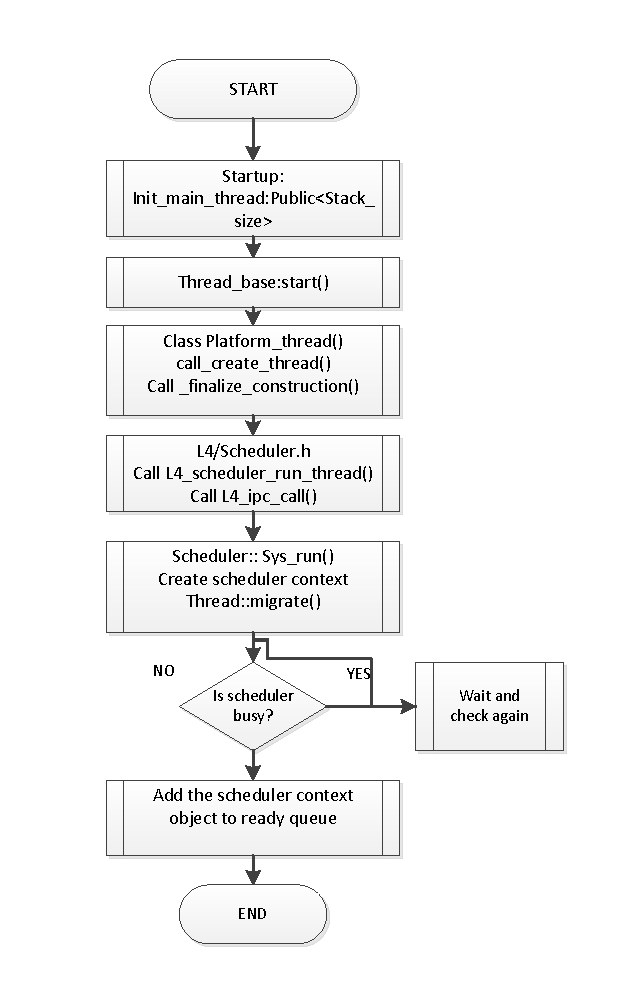
\includegraphics[width=0.7\linewidth]{figures/Thread_creation}
\caption{Thread creation calls in Genode operating system}
\label{fig:Thread_creation}
\end{figure}

Thread creation in a Genode application is done by creating a class and inheriting the Genode \texttt{Thread} class. This class takes the stack size as a template parameter. Figure \ref{fig:Thread_creation} shows the sequence of calls that take place between the application and the kernel. The derived class needs to have a constructor and an entry function. The entry function implements the work done by the thread. When the thread objects are created and the start method of the Genode Thread class is called, the entry method starts executing. The code listing \ref{threadcreate} shows the inheritance of the Thread class to create user threads.

\begin{lstlisting}[caption={Thread creation class},label={threadcreate}, style=customcpp]
class Mythread : public Genode::Thread<2*4096>
{
	public:

		Mythread() : Thread("MyThread") { }

		void entry()
		{
			printf("I'm a thread\n");
			// Some useful work
		}
};
\end{lstlisting}

Once the Genode application creates the thread, the following sequence of calls takes place.

\begin{enumerate}
\item The kernel specific code takes over in the Genode. In case of Fiasco.OC, the call goes to \texttt{base-foc/src/core/Platform\_thread.cc}. Platform\_thread.cc implements the major functionalities to interact with the kernel, such as creating the thread, setting the thread related values and selecting the affinity space and priorities for the thread. Further, there are two types of platform\_thread constructors available. One for the core threads, which takes just the name of the argument and the other for user-level threads, which takes the name and priority of the thread.  The platform thread constructor calls \texttt{\_create\_thread} and \texttt{\_finalize\_construction }.

\item The \_create\_thread calls l4\_factory\_create\_thread API with the L4\_BASE\_FACTORY\_CAP and a thread's local ID. This call creates an L4 thread in the kernel. 

\item The \_finalize\_construction calls L4 APIs to create an IRQ, to set the name of a thread in kernel and to set the scheduling parameters (l4\_scheduler\_run\_thread).

\item \texttt{l4\_scheduler\_run\_thread} makes an IPC call to the scheduler kernel object, by which kinvoke call of the scheduler object is invoked.

\item The sys\_run call identifies the thread and scheduling parameters associated with it. The scheduler\_context object is created with the defined scheduling strategy (FP or EDF). The thread is then migrated to the corresponding CPU and added to the ready queue.  
\end{enumerate}

\section{Creating a Kernel Object in Fiasco.OC}\label{implement:kernelobject}
In this section, creating a new kernel object is explained. This object can be utilized to make dedicated work in the kernel. The following changes are required to create a kernel object and compile it. A new class should be created, which inherits \texttt{Icu\_h<object name>} and
\texttt{Irq\_chip\_soft} classes. The class has to declare this as a kernel object using a macro (FIASCO\_DECLARE\_KOBJ()) provided by the Fiasco.OC. The memory is allocated outside the class by defining the kernel object and sending the class name as a parameter. The class has to have a static object created inside it and an interrupt request(Irq\_base) object defined. In the constructor of the class, it is important to register this object to the initial kernel objects. 

The class definition and the registration of the kernel object can be seen in Listing \ref{kobject}. The new object is called \texttt{RQ\_manager}, which should take care of the ready queue handling.

\begin{lstlisting}[caption={Creating new kernel object},label=kobject, style=customcpp]
class RQ_manager : public Icu_h<RQ_manager>, public Irq_chip_soft
{
  FIASCO_DECLARE_KOBJ();
  typedef Icu_h<RQ_manager> Icu;

public:
  enum Operation
  {
	RQ_info = 0,
	Schedule_thread = 1,
  };

  static RQ_manager rq_manager;
private:
  Irq_base *_irq;
};

FIASCO_DEFINE_KOBJ(RQ_manager);

PUBLIC inline
RQ_manager::RQ_manager() : _irq(0)
{
  initial_kobjects.register_obj(this, 8);
}

PUBLIC
L4_msg_tag
RQ_manager::kinvoke(L4_obj_ref ref, L4_fpage::Rights rights, Syscall_frame *f,
                   Utcb const *iutcb, Utcb *outcb)
{
}

enum Protocol{
  Label_rq_manager = -22L,   // Protocol ID for rq manager objects<l4_types.cpp>
}
enum l4_msgtag_protocol{
L4_PROTO_RQ_MANAGER = -22L, //Protocol for messages to a rq_manager object<types.h>
}

static Cap_index const C_rq_manager = Cap_index(8); //kernel-thread-std.cpp
\end{lstlisting}

This class implements methods from the inherited classes, such as \texttt{icu\_bind\_irq} and \texttt{icu\_set\_mode} and a \texttt{kinvoke} call. The \texttt{kinvoke} call is then used by the Fiasco.OC objects for interprocess communication.

This created kernel object needs to be associated with a protocol ID. These protocol IDs are used for kernel implemented objects and are assigned in the protocol section of the l4\_msg\_tag in \texttt{l4\_types.h}.